\documentclass[a4paper]{article}

\usepackage[english]{babel}
%\usepackage[utf8x]{inputenc}
\usepackage{amsmath}
\usepackage{graphicx}
\usepackage[colorinlistoftodos]{todonotes}
\usepackage[all]{xy}
\usepackage{dsfont}
\usepackage{amssymb}
\usepackage{bbold}
\usepackage{amsthm}

\usepackage{tikz}
\usepackage{verbatim}
\usetikzlibrary{matrix}
\usetikzlibrary{cd}

\usepackage[autostyle=true]{csquotes}
\usepackage{pdfpages}
\usepackage{hyperref}
\usepackage{fancyhdr}


\newtheorem{theorem}{Theorem}[section]
\newtheorem{proposition}{Proposition}[theorem]
\newtheorem{lemma}{Lemma}[theorem]
\newtheorem{corollary}{Corollary}[theorem]
\newtheorem*{definition}{Definition}


\newcommand{\norm}[1]{\left\lVert#1\right\rVert}

\newcommand{\Rn}{\mathbb{R}^n}
\newcommand{\Rr}{\mathbb{R}}


\newcommand{\too}[1]{\overset{#1}{\longrightarrow}}
\newcommand{\hookar}[1]{\overset{#1}{\hookrightarrow}}
\newcommand{\colim}[1]{ \underset{#1}{\texttt{colim}} \text{ } }
\newcommand{\fset}[1]{ \{ #1_0 , \dots , #1_n \} }
\newcommand{\ddt}{\frac{d}{dt}}


\newcommand{\N}{\mathbb{N}}
\newcommand{\Z}{\mathbb{Z}}





\title{Laboratorio 2}
\date{}
\fancyhead[L]{Universidad Finis Terrae \\ Facultad de Ingeniería \\ Algebra Lineal \\ 1er semestre de 2025}
\fancyhead[R]{\includegraphics[scale=0.1]{UFT.png}}

\begin{document}

\maketitle
\thispagestyle{fancy}

\textbf{Marco Teórico:}
\vspace{0.2 cm}

\textbf{Valor Propio:} Un \textit{valor propio} de una matriz $A$ de tamaño $n \times n$ corresponde a un escalar $\lambda \in \Rr$ para el cual existe un vector $v \in \Rn$ tal que
$$ Av= \lambda v $$

Un vector que cumple esto se llama \textit{vector propio} asociado al valor propio $\lambda$.

Una matriz de tamaño $n \times n$ tiene a lo más $n$ valores propios reales. Usaremos estos valores propios para estudiar el comportamiento de una red social. Para esto necesitamos la llamada \textit{matriz laplaciana}, la cual guarda la información sobre las conexiones entre vértices de un grafo, así como el grado de cada vértice. 

\textbf{Grado de un vértice:} El \textit{grado} de un vértice corresponde al número de conexiones que tiene, por ejemplo en el siguiente grafo
\begin{center}
    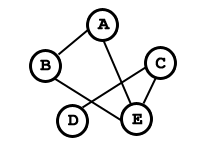
\includegraphics[scale=0.4]{grafo1.png}
\end{center}
El vértice $B$ tiene grado $2$, mientras que el vértice $E$ tiene grado $3$. 

\textbf{Matriz Laplaciana:} La \textit{matriz laplaciana} de un grafo $G$ con vértices $v_1, \dots , v_n$ es una matriz $L=(L_{i,j})$ de tamaño $n \times n$, donde

\[L_{ij}=\left\{ \begin{array}{ll}
     gr(v_i) & \text{ si } i=j  \\
     -1 & \text{ si existe arista entre } v_i \text{ y } v_j, \\
    0 & \text{ en otro caso }
\end{array}\right.\]
En otras palabras, $L=D-A$, donde $A$ es la matriz de adyacencia (ver lab1), y $D$ es una matriz diagonal, cuyos valores en la diagonal corresponden con los grados de los vértices.

El tamaño de los valores propios de una matriz laplaciana contiene información valiosa sobre el grafo.
\begin{itemize}
    \item El valor propio más pequeño $\lambda_1$ de la matriz laplaciana se conoce como el "valor propio de conectividad" y está relacionado con la existencia de componentes desconectados en la red. Si $\lambda_1=0$ entonces la red es conexa, mientras que si $\lambda_1>0$, la red tiene componentes desconectados.
    
    \item El segundo valor propio más pequeño de la matriz laplaciana se conoce como el "valor propio de expansión" y está relacionado con la capacidad de la red para propagar información. Si este valor propio es grande, entonces la red es más propensa a la propagación de información.

    \item Los valores propios de la matriz laplaciana también están relacionados con la robustez de la red frente a la eliminación de vértices, ya que los vectores propios asociados a los valores propios más grandes de la matriz dan información sobre los vértices más críticos para la estructura y la dinámica de la red.

    \item Los valores propios de la matriz laplaciana también pueden usarse para identificar comunidades o grupos de nodos en la red, ya que los vectores propios correspondientes a los valores propios más grandes pueden usarse para agrupar nodos que tienen una alta similitud o cercanía entre sí.
    
\end{itemize}

\newpage
\textbf{Problema a resolver:}
\vspace{0.2 cm}

Los siguientes tres grafos representan interacciones en una red social

\vspace{0.2 cm}
\textbf{Grafo 1:}
\begin{center}
    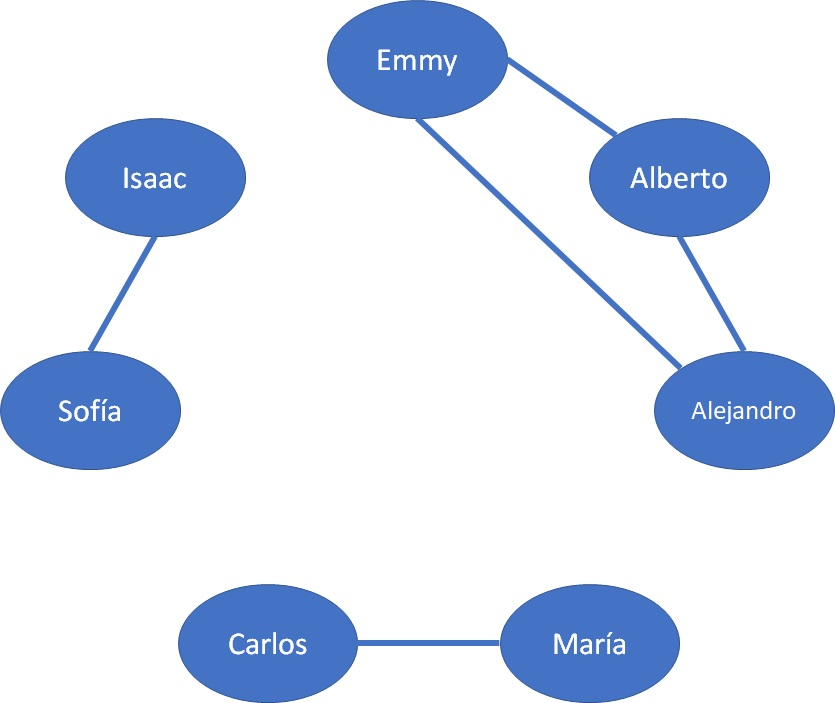
\includegraphics[scale=0.3]{Grafo Lab2_1.jpg}
\end{center}

\textbf{Grafo 2:}
\begin{center}
    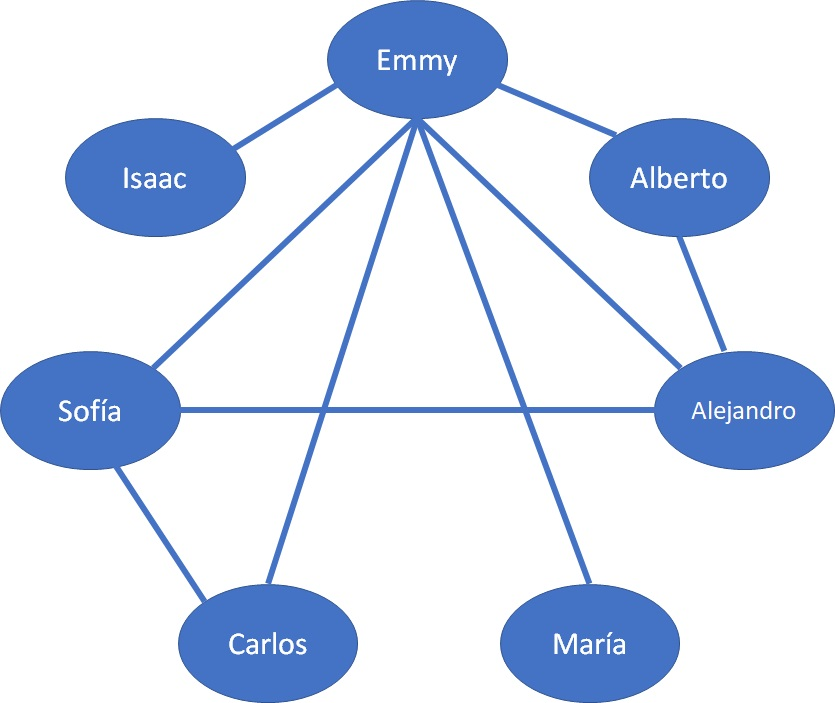
\includegraphics[scale=0.3]{Grafo Lab2_2.jpg}
\end{center}

\textbf{Grafo 3:}
\begin{center}
    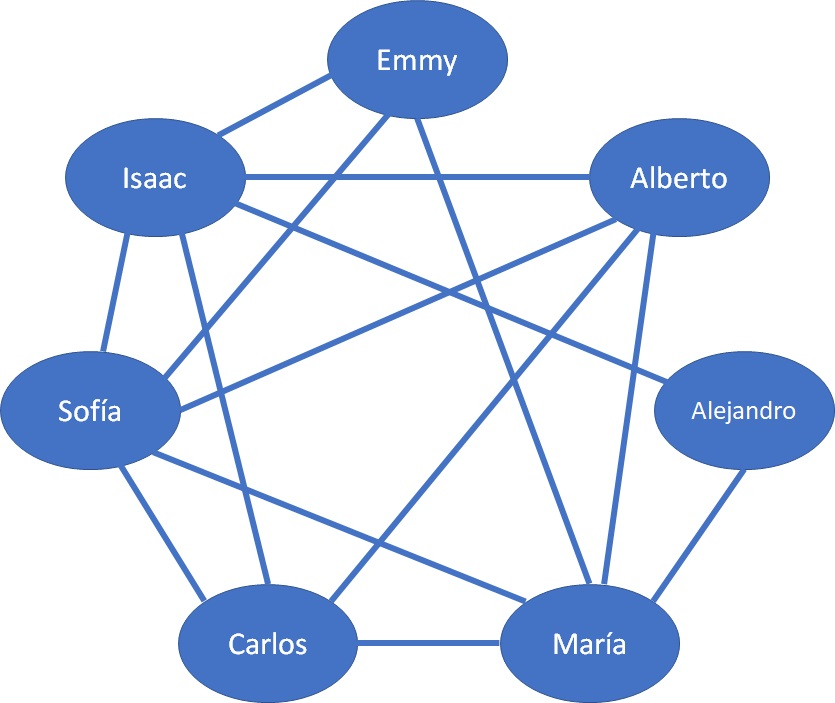
\includegraphics[scale=0.3]{Grafo Lab2_3.jpg}
\end{center}

Vamos a analizar la información que entregan las matrices laplacianas de este grafo, utilizando los valores y vectores propios de cada matriz.

\begin{enumerate}
    \item Numere a las personas de la forma que mejor le parezca, luego obtenga la matriz laplaciana correspondiente a cada grafo.
    
    \item Obtenga los valores propios de cada matriz laplaciana, junto con vectores propios asociados. Puede ayudarse con la función \textit{eig} de Matlab.

    \item Analice en cada matriz, el valor propio cuyo valor absoluto sea el más pequeño, ¿Qué le dice sobre los grafos? Si considera \textbf{solamente} la información dada por este valor propio, ¿Qué puede decir sobre la propagación de un rumor en cada red social?

    \item Analice en cada matriz, el valor propio cuyo valor absoluto sea el segundo más pequeño. Compare los valores en cada matriz ¿Qué información nos da sobre la propagación de información en los grafos? Mirando el dibujo de cada grafo, ¿Cómo se refleja la información otorgada por este valor propio? (por ejemplo, si un valor propio dio información de que la información se propaga rápido, ¿Qué explicación puede dar para esto, desde el dibujo?)

    \item Considere ahora el valor propio de valor absoluto más grande, y el vector propio asociado. El tamaño de cada coordenada del vector tiene información sobre la importancia del vértice correspondiente a esa coordenada. ¿Qué información le da sobre los vértices de los grafos? ¿Cómo ve esto en la representación gráfica de los grafos? ¿Cómo influye esta información a la hora de lanzar una propaganda? Puede ayudarle en esto analizar el segundo grafo. 
    
    \item ¿Cuál de los grafos presentados recomendaría para el marketing de un producto? ¿Por qué? ¿Qué estrategia utilizaría? ¿Cómo se relaciona su decisión con la información entregada por los valores y vectores propios?

    %\item ¿Qué sugerencias podrían hacer para mejorar la conectividad, la propagación de información o la robustez de cada red social, en base a los resultados obtenidos a partir de los valores propios de la matriz laplaciana?
    
\end{enumerate}

\newpage
\textbf{Aspectos formales del Laboratorio}
{\bf{Grupos de Trabajo}:} Los grupos de trabajo estarán conformados por 3 o 4 estudiantes y
deben ser aprobados por el profesor. Se penalizarán las modificaciones posteriores de
estos grupos y cualquier problema que se le presente al profesor relacionado con los
mismos.
\vspace*{.5cm}

Todas las entregas se deben realizar en el portal e-Finis en los buzones habilitados para
tal efecto, no se aceptan trabajos enviados por correo. 

\vspace*{.5cm}

\noindent{\bf{Formato de Entrega}}
Se deben entregar los documentos en PDF (en caso contrario no se corregirá el informe)
en formato \LaTeX  con el formato entregado por su profesor.



{\bf{NOTA}}
La copia y/o plagio serán sancionados de acuerdo a lo estipulado en el Reglamento de la
Universidad.
\end{document}